\Needspace{10\baselineskip}
\section{作品概述}
\label{sec:overview}

\subsection{功能与特性}
EdgeSight 面向受控工位的螺栓、螺母、垫圈识别与检查。
真实 HDMI 相机提供画面；板卡完成预处理、目标定位与分类；自研 RISC-V 核按工单汇总判定；PS 提供结果与配置通信；网页端展示视频、目标框、类别与检查结论。
首版功能包括按类别计数、工单核对（缺件、多余件、错料）、一次检查一条批次记录、异常截图与记录导出、设备连接与推理状态诊断。

\subsection{应用领域}
紧固件工业检查。
工位背景简单、稳定可控、照明理想；物体自由摆放且互不遮挡。
实际支持范围由采样验证，阴影、反光、接触与遮挡不在首版范围内，超条件时提示复检。

\subsection{主要技术特点}
三个自研数字模块共存于同一片可编程逻辑：RISC-V 处理器核、HDMI 视觉预处理流水线、INT8 CNN 推理协处理器。
接口以冻结契约为准；每一级实现都有仓库内的黄金参考与回归入口。
性能口径区分外推、实点与板上三档，不做无证据声明。

\subsection{主要性能指标}
表~\ref{tab:keymetrics} 汇总关键指标，每行标注口径日期；依据见对应参考文献。

\begin{table}[H]\centering\small
\caption{主要性能指标与口径}\label{tab:keymetrics}
\begin{tabularx}{\linewidth}{@{}P{30mm}Y P{20mm}@{}}\toprule
指标 & 数值与口径 & 日期\\\midrule
处理器核 & v1 三级流水、三路转发、Radix-4 乘除、可切换 BHT & 2026-09-27\\
CoreMark & CPI 1.886（无转发）$\rightarrow$ 1.606（转发+BHT2），retired 10{,}106{,}386 & 2026-10-07\\
架构测试 & riscv-arch-test I+M 子集 44/44 签名匹配 & 2026-10-07\\
核时序 & OOC 实点 86.806 MHz（BHT2 @ 11.52 ns，WNS +0.538 ns） & 2026-10-07\\
最小 SoC & 40 MHz 上板，LED 判据；LUT 6{,}768、BRAM 8、DSP 0 & 2026-10-07\\
视觉链路 & 720p60；\code{video_pipeline} OOC WNS +0.330 ns & 2026-10-27\\
协处理器 & 128 MAC INT8；整网 472{,}593 拍；DSP 136/220、BRAM36 69/140 & 2026-10-15\\
整机门禁 & WNS +2.078 ns（A 包，含协处理器） & 2026-10-27\\
板上 CNN & zero/pattern 各 3 轮 6/6 匹配；四例黄金全匹配 & 2026-10-26\\
多目标实板 & 12 轮 85 个结果与整数参考逐项一致（CNN r6） & 2026-10-28\\\bottomrule
\end{tabularx}\end{table}

\subsection{主要创新点}
在同一片 FPGA 内完成感知、推理与调度的全自研闭环：视觉预处理、INT8 协处理器与自研 RISC-V 核分工协作，不依赖第三方处理器软核。
建立契约先行与逐位黄金对拍的质量体系：量化网络、流水线时序与推理结果都有独立参考。
把大模型协作制度化为理解门槛与证据目录，AI 产出经讲解、答题与独立审查后才入库。

\subsection{设计流程}
设计按八阶段推进：需求与验收、接口契约、RTL 与模块 tb、全量回归、综合与时序、上板 bring-up、软件联调、证据归档（图~\ref{fig:flow}）。
每阶段以门禁与仓库内脚本收口；仿真、软件、板上三级别分别标注，不用低级别证据替代高级别结论。

\begin{figure}[H]\centering
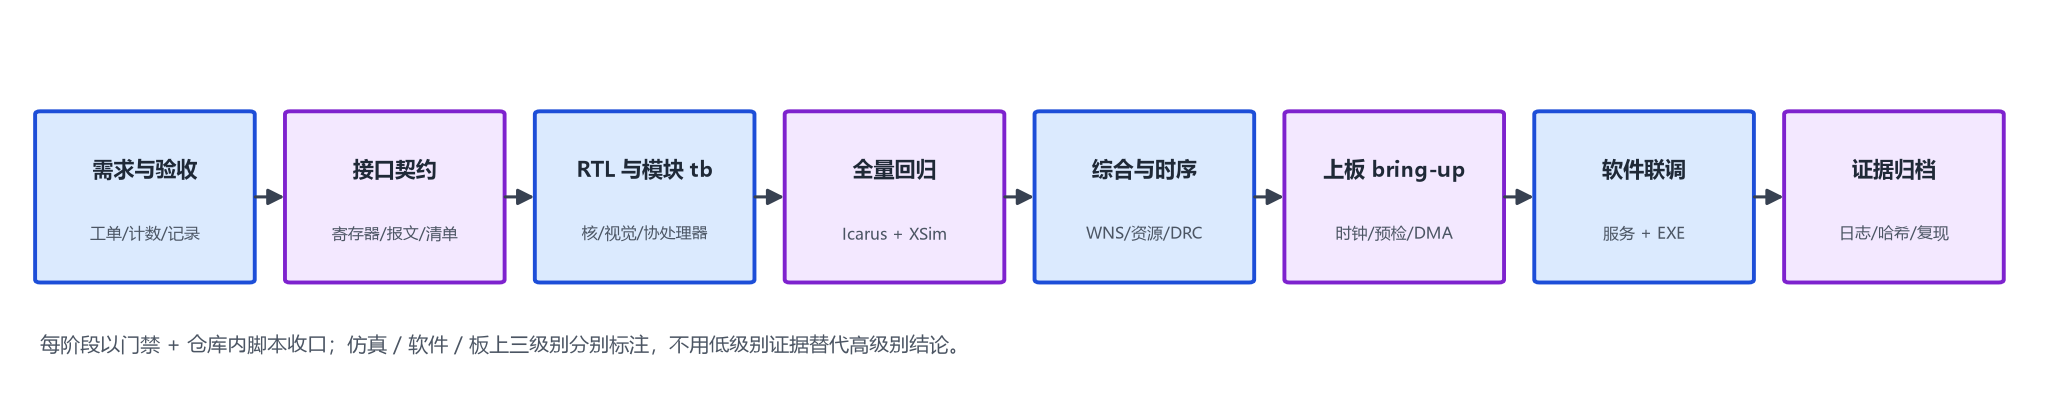
\includegraphics[width=0.98\linewidth]{fig_flow.png}
\caption{设计流程八阶段与门禁收口（仓库配图）}\label{fig:flow}
\end{figure}
